%&tex
\chapter{Prerequisites on Learning Disentanglement}\label{sec:prerequisites}



\section{Learning from Data}
	{Learning from data} is commonly understood as the ability of algorithms to improve their performance on a task with experience accumulated from the observation of data \cite{goodfellow16dlb}. The source of data is usually a dataset - set of data points $X = \{x_i | i \in \{1\ldots n\} \}$, which are sampled from a probability distribution $x_i \sim p(x)$.
	In general, these data points are multi-dimensional. In computer vision in particular, data are images $\mathbf{x}$ with height $h$ and width $w$, so that the data points are $\mathbf{x} \in \mathbb{R}^{h \times w}$.

	\subsection{Supervised}\label{sec:supervised}
		The term {supervised learning} denotes the task to learn a mapping from data points $x_i$ to target labels $y_i$.
		A supervised algorithm has access to data-label pairs  $(y_i, x_i) \sim p(y, x)$, in order to estimate the connection between data points and labels, either in form of a conditional probability $p(y|x)$, or in form of a deterministic function $y = f(x)$.
		The label $y$ can be either discrete (\eg information about an object class) or continuous (\eg the location of an object part in an image).
		Recent advances, in particular the effectiveness of neural network models (cf. Sec. \ref{sec:neuralnetworks}) on big datasets, have led to huge progress on problems that can be formulated as regression or classification. That is why on many traditional computer vision problems, such as object recognition, image classification or human pose estimation, machines are now performing on a superhuman level; hence, these problems are now considered to be essentially solved.\\
		The Achilles' heel of supervised learning lies in the need for a viable supervision signal. To get labels, it is usually required to manually annotate the data. The human effort in this is costly, error-prone and not scalable to the ever-growing vast amounts of raw data.

	\subsection{Unsupervised}\label{sec:unsupervised}
		{Unsupervised learning} is the endeavour to learn about structures and patterns in unlabelled data. In this paradigm, the learning algorithm has access to the samples of the data distribution $x \sim p(x)$. The task is usually framed as a form of density estimation, \ie to model the entire distribution in a probabilistic generative model (cf. Sec. \ref{sec:genmodel}).
		Unsupervised learning is considered much harder than supervised learning \cite{bishop06pattern}. There are several complications in the design of unsupervised algorithms:
		\begin{itemize}
			\item Naturally, without supervision, \textit{the goal of learning is not specified}, hence surrogate objectives have to be formulated. The lack of specification renders the evaluation oftentimes arbitrary and subjective~\cite{theis15evalgen}.
			\item It is a priori not clear, \textit{how much prior knowledge} should be embedded. To introduce no artificial bias, some argue for a purely data-driven approach. Others argue for the importance of certain inductive priors to guide learning \cite{tenenbaum18think}.
			A related modeling choice is, whether the algorithm should be model-free or model-based\todo{ cite huszar article}.
			% \note{model-free vs model-based approaches:}
			% \note{model-based $\rightarrow$ more flexible, transferable, allows for modular combination (like parts)}
			In this work we argue for using more prior knowledge and modelling assumptions to obtain strong constraints.
			\item Lastly, the \textit{definition of the term unsupervised} itself is subject to discussion. What entitles an algorithm to be called unsupervised? While the definition itself has no practical importance, unclear and imprecise terminology unnecessarily confuses.



		\end{itemize}
		\todo{connection between unsupervised and supervised learning, \cite{goodfellow16dlb}.}
		\note{A possible framing of the goal is data compression.}
		\note{e.g. outlier detection where $p(x)$ has low probability}
		\note{What does unsupervised even mean? No prior assumptions, no knowledge at all? Unspecified.. read on this.}
		\note{notion of truly unsupervised learning is actually harmful to progress.}

	\subsection{Artificial Neural Networks}\label{sec:neuralnetworks}

		\begin{figure}[htp]
			\centering
			\usetikzlibrary{positioning}
			\tikzset{%
			  every neuron/.style={
			    circle,
			    draw,
			    minimum size=1cm
			  },
			  neuron missing/.style={
			    draw=none,
			    scale=4,
			    text height=0.333cm,
			    execute at begin node=\color{black}$\vdots$
			  },
			}

			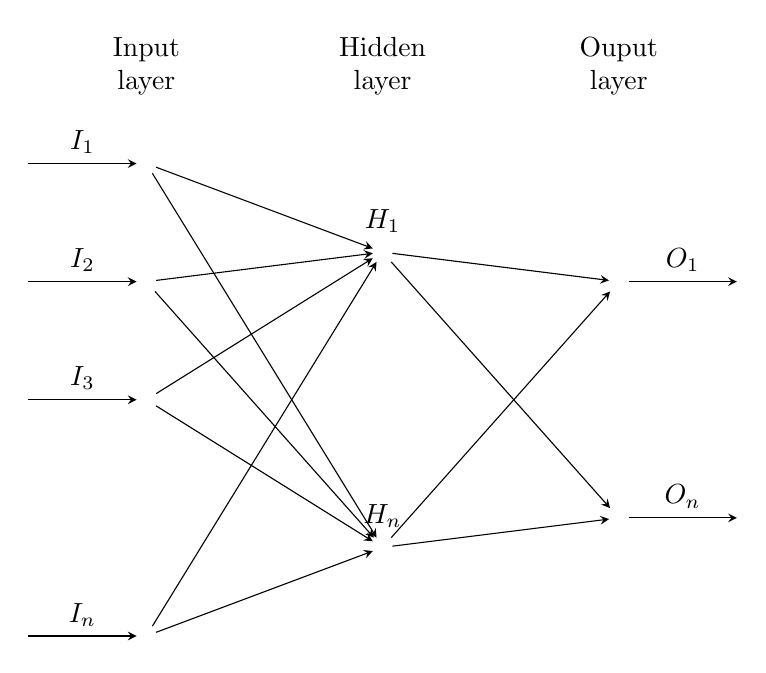
\begin{tikzpicture}[x=1.5cm, y=1.5cm, >=stealth]
				\foreach \m/\l [count=\y] in {1,2,3,missing,4}
				  \node [every neuron/.try, neuron \m/.try] (input-\m) at (0,2.5-\y) {};

				\foreach \m [count=\y] in {1,missing,2}
				  \node [every neuron/.try, neuron \m/.try ] (hidden-\m) at (2,2-\y*1.25) {};

				\foreach \m [count=\y] in {1,missing,2}
				  \node [every neuron/.try, neuron \m/.try ] (output-\m) at (4,1.5-\y) {};

				\foreach \l [count=\i] in {1,2,3,n}
				  \draw [<-] (input-\i) -- ++(-1,0)
				    node [above, midway] {$I_\l$};

				\foreach \l [count=\i] in {1,n}
				  \node [above] at (hidden-\i.north) {$H_\l$};

				\foreach \l [count=\i] in {1,n}
				  \draw [->] (output-\i) -- ++(1,0)
				    node [above, midway] {$O_\l$};

				\foreach \i in {1,...,4}
				  \foreach \j in {1,...,2}
				    \draw [->] (input-\i) -- (hidden-\j);

				\foreach \i in {1,...,2}
				  \foreach \j in {1,...,2}
				    \draw [->] (hidden-\i) -- (output-\j);

				\foreach \l [count=\x from 0] in {Input, Hidden, Ouput}
				  \node [align=center, above] at (\x*2,2) {\l \\ layer};
			\end{tikzpicture}

			\caption{Sketch of artificial neural network model}
			\label{fig:overview}
		\end{figure}
		Artificial neural networks are a powerful and flexible tool for function approximation. Inspired by biological neurons, there have been numerous questionable claims \wrt their biological plausibility. % cite bishop
		Here, we will treat an artificial network solely as a parametric non-linear function approximator. They can approximate a function $y = f(x)$ with vector input $x = \{ x_i | i = 1 \ldots n \}$ and vector output $y = \{ y_j | j = 1 \ldots m \}$:
		\begin{equation} \label{eq1}
			\begin{split}
				h_j & =  a (\sum_i w_{ji} x_i + w_{0i})  \\
				y_j & =  a' (\sum_i w'_{ji} h_i + w'_{0i})
			\end{split}
		\end{equation},
		with weight matrices $w, w'$, non-linear so-called activation functions $a, a'$  and bias vectors $w_{0}$, $w_{0}'$.
		Typical activation functions are for example the sigmoid function ($a_{sigm}$ or the rectified linear unit ($a_{relu}$):
		\begin{equation}
			a_{\textrm{sigm}}(x)= \frac{1}{1+e^{-x}}
		\end{equation}
		% \begin{equation}
			% a_{\textrm{tanh}}(x)= \frac{2}{1+e^{-2x} -1 }
		% \end{equation}
		\begin{equation}
			a_{\textrm{relu}}(x)=
			\begin{cases}
			      0 & x\leq 0 \\
			      x & x > 0
			\end{cases}
		\end{equation}
		% \begin{equation}
			% a_{\textrm{elu}}(x)=
			% \begin{cases}
				% e^{-x}-1  & x\leq 0 \\
			      % x & x > 0
			% \end{cases}
		% \end{equation}
		The activation function needs to be non-linear, otherwise the neural network is just a linear classifier (matrix multiplies are again matrices).
		% multiple layers
		The components $h_j$ are called hidden units or neurons. Neural networks can also comprise multiple hidden layers via $h_j  =  a (\sum_i w_{ji} h_i + w_{0i})$.
		It can be shown, that in the limit of infinite hidden units $h_j$ they can approximate any (continuous) function arbitrarily close \cite{cybenko89approx, hornik91approx}.
		In practice, however, networks with more that one layer, referred to as deep neural networks, seem to work better. This may be due to the possibility of building a hierarchical feature representation \cite{zeiler14vis}, that reflects the hierarchical nature of the physical reality. % cite tegmark
		% convolutional
		For processing image data, the weight matrices can be constrained to be only locally connected and to share weights across locations to enforce translation invariance, resulting in \textit{convolutional} neural networks.

		% optimization
		Deep neural networks have highly non-convex likelihood functions, hence for optimization iterative numerical methods are used: The weights $w$ are initialized to some initial value $w^0$% cite glorot
		and then updated ($w^{t+1}\rightarrow w^t$).
		A simple yet successful update rule is gradient descent,
		\begin{equation}
			w^{t+1} = w^{t} - \lambda \nabla_{w^t}	 \mathcal{L} (w^t).
		\end{equation}
		In practice, calculating derivatives of the likelihood \wrt the weights can be done efficiently via error backpropagation.
		For big datasets %(cite lecun)
		one usually approximates the gradient on a random subset of the data, which renders the optimization stochastic.


\newpage
\section{Generative Models}\label{sec:genmodel}
	\begin{quote}
	    What I cannot create, I do not understand. - R. Feynman
	\end{quote}
	Learning and understanding structure in data by being able to generate, is the rationale behind generative modelling.
	Generative models are mostly applied for unsupervised learning and can be contrasted to discriminative models. While discriminative models are used to model posterior conditionals $p(y|x)$ (\eg for supervised learning (cf. Sec. \ref{sec:supervised}), generative models capture the complete data distribution $p(x)$ in an estimate $\hat p(x)$ \cite{bishop06pattern}. Thus, after estimation, one can generate samples from this model $\hat p$. Hence the name generative model.
	\note{Generative modeling can be used for outlier search, where regions with low probability under the model are taken as indicative for an outlier.}
	The currently predominant generative models are built on either autoencoding or adversarial formulations:

	\subsection{Autoencoding Formulations}\label{sec:autoencoding}
		An autoencoding model is learning by reconstructing samples of data, $\hat x = f(x)$. To enforce data compression (otherwise the identity function is a trivial solution of autoencoding) the function has an information bottleneck, namely an inferred latent code $z$ of reduced dimension. The autoencoder is then the chain of an encoding function $z = e(x)$ and a decoding function $\hat x = d(z) = d(e(x))$.

		Whereas the conventional autoencoder consists of deterministic mappings $e, d$, the {variational autoencoder} \cite{kingma13vae} models the probability distribution $p(x)$. More specifically, it maximizes a lower bound to the logarithmic likelihood $\log p(x)$ of data $x$. This so-called variational lower bound $\mathcal{L}$ is given by:
		% \begin{equation}\label{eq:vae}
			% \mathcal{L} = \underbrace{\mathds{E}_{z\sim q(z|x)}  \log p(x|z)}_{\textrm{reconstruction loss}}  - \underbrace{\textrm{KL}(q(z|x)||p(z))}_{\textrm{regularization}}
		% \end{equation}
		\begin{equation}\label{eq:vae}
			% \mathcal{L} = \mathds{E}_{z\sim q(z|x)}  \log p(x|z) - \textrm{KL}(q(z|x)||p(z))
			\mathcal{L} = \mathds{E}_{z\sim q(z|x)}  \log p(x|z) - \mathds{E}_{z\sim q(z|x)} \log \frac{q(z|x)}{p(z)}
		\end{equation}

		Where $z$ introduces latent variables, with a prior distribution $p(z)$, with an approximation to the posterior $q(z|x)$ of the latent variables, and the posterior of the data given the latent variables $p(x|z)$. If one wants to model the distributions with neural networks, one typically uses Gaussian distributions and lets the networks predict the parameters (mean $\mu$ and variance $\Sigma$) based on the image.
		In the current machine learning contexts, all functions ($e, d$) and moments ($\mu, \Sigma$) are modelled with neural networks.

	\subsection{Adversarial Formulations}\label{sec:adversarial}
		{Generative adversarial networks} (GAN) \cite{goodfellow14gan} consist of two neural networks competing in a zero-sum game. A generator network $G$ is generating images based on a latent code $z$ sampled from a distribution $p(z)$. The discriminator network $D$ is a binary classifier with the task to classify an image as originating from the data distribution $p_{\mathrm{data}}$ or from the distribution produced by $G$. The loss function of $G$ is the negative of the loss of $D$, such that one can formulate the optimization in a minmax form:
		\begin{equation}
			% \begin{split}
			\min_D \max_G - \frac{1}{2} \mathds{E}_{x \sim p_{\mathrm{data}}} [\log D(x)] - \frac{1}{2} \mathds{E}_{z\sim p(z)}[\log (1-D(G(z)))]
			% \end{split}
		\end{equation}
		The generator is then optimized to make the output indiscriminable from the data distribution.
		The discriminator can be interpreted as a learned similarity metric, to measure the closeness of an image to the data distribution \cite{larsen15vaegan}.
		There are many variants and extensions to this basic principle of learning with an adversarial task. For example, one can learn a discriminator for a set of image patches \cite{isola17image2image}. \todo{find more examples, of the gan zoo}

\section{Disentangling Representations}\label{sec:disentangled}
	In supervised learning, a performance measure is naturally induced by the metric, that is being optimized. In the unsupervised setting, judging the performance of a model is less straightforward.
	How to rate the quality of the latent representation?
	\note{For example, when modelling an image domain, one could subjectively rate the quality of the generated image.}
	\todo{introduce latent representation in data compression framing }

	\subsection{Learning Representations}

	\begin{quote}
		{Disentangle as many factors as possible, discarding as little information about the data as is practical.} - Bengio \etal \cite{bengio13rep} % Y. Bengio, A. Courville and P. Vincent \cite{Bengio2013rep}
	\end{quote}

	According to Bengio \etal \cite{bengio13rep}, a representation is useful, if it can be applied to many - in advance unknown - different tasks, while being trained on only one particular task.
	As the downstream tasks can be multifarious, the essential \textit{information} should be contained in the representation.
	For some tasks only a subset of aspects of the data will be necessary, that is why \textit{disentangled factors} make a representation particularly practical.

	The latent representation $z$ learned by generative models captures the essential \textit{information} of the data distribution. That is made sure by requiring the ability to generate samples from the original data distribution from it.
	How then to reach the second goal, the \textit{disentanglement} of generative factors?

	\subsection{Disentangling by Equivariance and Invariance}
		\begin{figure}[htp]
			\centering
			% \begin{tikzpicture}
	% % Define nodes
	% \node[obs]                               (x) {$\mathbf{x}$};
	% \node[latent, above=of x, xshift=-1.3cm] (z1) {$\mathbf{z_1}$};
	% \node[latent, above=of x, xshift=1.3cm]   (zn) {$\mathbf{z_N}$};
	% \node[latent, above=of x]   (zi) {$\mathbf{z_i}$};
	% \node[auto=false, above=of x, yshift=0.2cm, xshift=0.7cm] (dots) {$\cdots$}  ;
	% \node[auto=false, above=of x, yshift=0.2cm, xshift=-0.6cm] (dots1) {$\cdots$}  ;
%
	% \node[latent, below=of x, xshift=-1.3cm] (ez1) {$\mathbf{\hat z_1}$};
	% \node[latent, below=of x, xshift=1.3cm]   (ezn) {$\mathbf{\hat z_N}$};
	% \node[latent, below=of x]   (ezi) {$\mathbf{\hat z_i}$};
	% \node[auto=false, below=of x, yshift=0.2cm, xshift=0.7cm] (dots2) {$\cdots$}  ;
	% \node[auto=false, below=of x, yshift=0.2cm, xshift=-0.6cm] (dots3) {$\cdots$}  ;
%
	% \edge {z1,zi,zn} {x} ; %
	% \edge {x} {ez1,ezi,ezn} ; %
	% % Plates
	% % \plate {yx} {(x)(y)} {$N$} ;
	% % \plate {} {(w)(y)(yx.north west)(yx.south west)} {$M$} ;
% \end{tikzpicture}
\begin{tikzpicture}
	% Define nodes
	\node[obs]                               (x) {$\mathbf{x}$};
	\node[latent, above=of x, xshift=-1.3cm] (z1) {${z_1}$};
	\node[latent, above=of x, xshift=1.3cm]   (zn) {${z_N}$};
	\node[latent, above=of x]   (zi) {${z_i}$};
	\node[auto=false, above=of x, yshift=0.2cm, xshift=0.7cm] (dots) {$\cdots$}  ;
	\node[auto=false, above=of x, yshift=0.2cm, xshift=-0.6cm] (dots1) {$\cdots$}  ;

	\node[latent, below=of x, xshift=-1.3cm] (ez1) {$r_1$};
	\node[latent, below=of x, xshift=1.3cm]   (ezn) {$r_N$};
	\node[latent, below=of x]   (ezi) {$r_i$};
	\node[auto=false, below=of x, yshift=0.0cm, xshift=0.7cm] (dots2) {$\cdots$}  ;
	\node[auto=false, below=of x, yshift=0.0cm, xshift=-0.6cm] (dots3) {$\cdots$}  ;

	\edge {z1,zi,zn} {x} ; %
	\edge {x} {ez1,ezi,ezn} ; %
	% Plates
	% \plate {yx} {(x)(y)} {$N$} ;
	% \plate {} {(w)(y)(yx.north west)(yx.south west)} {$M$} ;
\end{tikzpicture}


			\caption{Disentangling causal factors means to infer an estimate - \ie a representation - from an image}
			\label{fig:infer}
		\end{figure}

		What is a factor? As outlined in the introduction (cf. Sec. \ref{sec:introduction}), factors in a representation should correspond to causal elements of the world.
		In general, these factors can interact in complicated ways to finally result in an image. Here, we only consider the case where multiple independent factors each have an influence (cf. Fig. \ref{fig:infer}):
		\begin{equation}\label{eq:independent}
			p(z_1 \ldots z_N) = \prod_i p(z_i)
		\end{equation}
		A change in an element, should then lead to: \emph{i)} a corresponding change in the representational factor and \emph{ii)} leave other factors, that represent other elements, unchanged.
		Formally, this can be seen as inference: a number of latent variables ${z_1}\ldots{z_N}$ interacted to cause the existence of the observed image $\mathbf{x}$. The task is now to infer estimates for these latent variables $r(\mathbf{x})_i:=r_i$. A graphical model of the process is shown in Fig.~\ref{fig:infer}.
		A disentangled representation should simultaneously fulfill equivariance and invariance: A change in ${z_i}$ should: \emph{i)} \textit{equivariantly} change in the abstract representational factor $r_i$, \emph{ii)} while leaving the other factors $r_j, j\neq i$, that represent other causes, \textit{invariant}.
		\todo{mathematically,.. $f \circ g (x) = ... $}
		\todo{draw other: arbitrary causal}
		\todo{incorporate definition~\cite{higgins18defdisrep}}


\section{Theoretical Impediments from Causality}\label{sec:causality}


	Generative factors represent causal elements.
	Learning a disentangled representation of generative factors is then understood as causal inference.
	In accordance with the causal literature~\cite{pearl18impediments}, we can make statements about the type of knowledge, that can be gained by the type of data provided. It turns out that from "raw" image data, it is actually impossible to learn a disentangled representation $z$ - raw data referring to images $x$ sampled from $p(x)$, without further assumptions.
	To elucidate this fact, we start with a primer for causal learning (Sec. \ref{sec:causallearning}), outline which inductive biases are needed for disentanglement (Sec. \ref{sec:requirements}) and assess how one can instantiate such biases for disentangling the factors of shape and appearance in images (Sec. \ref{sec:transform}, Sec. \ref{sec:anabysyn})).

	\subsection{Causal Learning}\label{sec:causallearning}
		\begin{figure}[htp]
			\begin{subfigure}{0.3\linewidth}
				\centering
				\begin{tikzpicture}
	% Define nodes
	\node[auto=false] (x) {}  ;
	\node[latent, below=of x, xshift=-1.3cm] (s) {$\mathbf{x}_1$};
	\node[latent, below=of x, xshift=1.3cm]   (a) {$\mathbf{x}_2$};
	\edge {s} {a} ; %
	% Plates
	% \plate {yx} {(x)(y)} {$N$} ;
	% \plate {} {(w)(y)(yx.north west)(yx.south west)} {$M$} ;
\end{tikzpicture}



				\caption{}
			\end{subfigure}
			\begin{subfigure}{0.3\linewidth}
				\centering
				\begin{tikzpicture}
	% Define nodes
	\node[auto=false] (x) {}  ;
	\node[latent, below=of x, xshift=-1.3cm] (s) {$\mathbf{x}_1$};
	\node[latent, below=of x, xshift=1.3cm]   (a) {$\mathbf{x}_2$};
	\edge {a} {s} ; %
	% Plates
	% \plate {yx} {(x)(y)} {$N$} ;
	% \plate {} {(w)(y)(yx.north west)(yx.south west)} {$M$} ;
\end{tikzpicture}



				\caption{}
			\end{subfigure}
			\begin{subfigure}{0.3\linewidth}
				\centering
				\begin{tikzpicture}
	% Define nodes
	\node[obs]                               (z) {$\mathbf{z}$};
	\node[latent, below=of x, xshift=-1.3cm] (x1) {$\mathbf{x}_1$};
	\node[latent, below=of x, xshift=1.3cm]   (x2) {$\mathbf{x}_2$};
	\edge {z} {x1,x2}; %
	% Plates
	% \plate {yx} {(x)(y)} {$N$} ;
	% \plate {} {(w)(y)(yx.north west)(yx.south west)} {$M$} ;
\end{tikzpicture}



				\caption{}
			\end{subfigure}
			\caption{Correlation implies causation - if $x_1$ and $x_2$ correlate, a) $x_1$ may cause $x_2$,  b) $x_1$ may be caused by $x_2$ or c) both are contingent on a latent cause $z$}
			\label{fig:reichenbach}
		\end{figure}

		Learning to infer causality is harder than statistical learning. We outline the basic problem for the case of two variables $x_1, x_2$: statistical learning aims at estimating probabilistic properties such as $p(x_1, x_2)$ or  $p(x_2|x_1)$ from data.
		It is a well-known theme in statistics is that correlation does not imply causation. Less well-known\todo{formulate differently} is Reichenbachs principle \cite{peters17elements, reichenbach56time}, that states: if two random variables are statistically dependent, then there exists a third variable that influences both or a direct causal link between them (Fig. \ref{fig:reichenbach}).
		In addition to estimating the probability distribution, also the causal structure has to be inferred \cite{peters17elements}.

		To show the limitations of raw data, we sketch an intuitive example problem (adapted from \cite{pearl18why}):
		How to learn the causal connection between a barometer and the weather? If the barometer is working well, there exists a clear correlation between the weather condition and the needle position. Given a dataset showing both barometer and corresponding weather condition, a capable machine learning algorithm will be able to capture this correlation. However, it will fail to understand the causal direction, since this is not possible from the data.
		Imagine how a human would go about solving this problem:
		Having a mechanistic model of the world he could reason about the precise causal mechanism relating weather to air pressure to needle position. A simple model could be: weather influences air pressure, pressure influences barometer needle position.
		What if one has no prior knowledge? A solution of child-level simplicity is, to force the needle to move with a finger. Without the power of magic, the weather will not change. Hence causality has to go other way or via a third latent variable influencing both \ie air pressure.
		% There cannot be an abstract intelligence, which finds out about the world purely by observation. The intelligence has to interact with the world, it has to be in the world.
		% e.g.  RCT
		To conclude, the strength of association (correlation) can be estimated with observational data alone, this can answer the question: how likely will it rain, if the barometer needle sinks? But not: how would the weather change if I force the barometer needle to sink?\todo{linking to next section}

		Pearl \cite{pearl18why} distinguishes between three types of questions, that can be answered by different types of knowledge:
		\begin{table}[htp]
			\centering
			\caption{Ladder of causation~\cite{pearl18impediments}. Questions at level $i$ of the ladder are only accessible with information from level $i$ or higher.}
			\label{tab:overview}
			\begin{tabular}{l|ccr}
				\hline
				Level & Symbol & Typical Activity & Typical Questions \\ \hline
				1. Association & $P(y|x)$ & Seeing & What if I see?  \\
				2. Intervention& $P(y|\mathrm{do}(x), z)$ & Doing& What if I do?  \\
				3. Counterfactual& $P(y_x|x', y')$ & Imagining & What if had done?  \\ \hline
			\end{tabular}
		\end{table}

		The levels of this \textit{ladder of causation} \cite{pearl18why, pearl18impediments} are separate not only conceptually, but in the type of data or assumptions that have to be made in order to access them. In particular, by unsupervised learning from observational data only the first level is accessible. The second level requires interactional data or model assumptions, while the third is inaccessible without an explicit model. The answers to these hypothetical questions (counterfactuals) lie by definition not in the data (facts).




	\subsection{Disentangling requires Interventions or Model Assumptions}\label{sec:requirements}
		The results from the study of causal inference also entail that "purely" unsupervised disentangling, \ie estimating $\mathbf{\hat z_i}$ from samples $x \sim p(x)$, is impossible. A proof for this can be found in \cite{locatello18challenging}.
		% so far fitting curve p(x) to data manifold
		Current machine learning operates mostly on the level of association, estimating (complex) correlations from raw data.
		As we have seen, this purely data-driven approach can only go so far.
		In contrast, humans seem to have the ability to interact with their environment and have innate assumptions on coherence, causality, physics etc., which introduce inductive priors~\cite{tenenbaum18think}.
		To bring \emph{i)} interventions and \emph{ii)} model assumptions to our problem of disentangling shape and appearance, we \emph{i)} apply changes to an image, which are assumed to change only one factor and \emph{ii)} model the causal process of the image generation in the theme of analysis-by-synthesis.
		\todo{math}
		% measure: p(x)
		% assume causal model: p(x | a, s)
		% want: p(s | x) and p(a | x)
%
% encoding
% $p(s | x )$
% $p(a | x) = p(a | s, x) p(s | x)$
%
% decoding
% $p(x) = p(x | a, s) p(a) p(s)$
%
% $p(x| do(s), do(a))$

	\subsection{Image Transformation as Intervention}\label{sec:transform}
		\begin{figure}[htp]
			\centering
			\begin{tikzpicture}
	% Define nodes
	\node[obs]                               (x) {$\mathbf{x}$};
	\node[latent, above=of x, xshift=-1.3cm] (s) {$\mathbf{s}$};
	\node[latent, above=of x, xshift=1.3cm]   (a) {$\mathbf{a}$};
	\node[latent, above=of s] (ts) {$\phi_\mathbf{s}$};
	\node[latent, above=of a] (ta) {$\phi_\mathbf{a}$};
	\edge {s,a} {x} ; %
	\edge {ts} {s} ; %
	\edge {ta} {a} ; %
	% Plates
	% \plate {yx} {(x)(y)} {$N$} ;
	% \plate {} {(w)(y)(yx.north west)(yx.south west)} {$M$} ;
\end{tikzpicture}



			\caption{An image $\mathbf{x}$ is assumed to be generated from the factors of shape $\sigma$ and appearance $\alpha$. Implementing an intervention with a transformation of factors, means changeing one factor without changing the other.}
			\label{fig:intervene}
		\end{figure}
		% $p(x| do(a), b)$
		To disentangle shape $\sigma$ and appearance $\alpha$, we can emulate interventions by image transformations. Under the assumption that certain transformations only lead to a change in shape, while leaving appearance invariant or vice versa, we obtain access to interventional data. %of the type x | s, a , x | do(s), a

	\subsection{Analysis-by-Synthesis to Model Assumptions}\label{sec:anabysyn}
		Additional assumptions can be made about the image generation process in the regime of analysis-by-synthesis:
		The key idea is, that the process of how an image is generated from underlying factors (graphics), is much better known that estimating the factors from the image (inverse graphics)\todo{ look up definition for inverse graphics}.
		One can combine a model for analysis and a model for synthesis to reconstruct an image (autoencoding, cf. Sec \ref{sec:autoencoding}).
		Herein the synthesis can be tightly constrained to fit the assumptions about reality \cite{tieleman14thesis}.
		Assumptions about how shape and appearance interact enable disentanglement. The idea to generatively entangle in order to disentangle has been explored before in other contexts~\cite{desjardins12genentangle}.

\todo{add shape and appearance}
\todo{objects}
